\documentclass{ximera}

\begin{document}
	\author{Stitz-Zeager}
	\xmtitle{Exercises for Root Radical Functions}{}

\mfpicnumber{1} \opengraphsfile{ExercisesforRootRadicalFunctions} % mfpic settings added 


In Exercises \ref{radicalgraphexfirst} - \ref{radicalgraphexlast},  given the pair of functions $f$ and $F$, sketch the graph of $y=F(x)$ by starting with the graph of $y = f(x)$ and using Theorem \ref{linearrootgraphs}.   Track at least two points and state the domain and range using interval notation.



% Transformed Exercises with Solutions

\begin{question}
$f(x) = \sqrt{x}$, $F(x) = \sqrt{x+3}-2$
\begin{solution}
$F(x) = \sqrt{x+3}-2$ \\ 

% \begin{mfpic}[15]{-5}{5}{-3}{5}
\axes
\tlabel[cc](5,-0.5){\scriptsize $x$}
\tlabel[cc](0.5,5){\scriptsize $y$}
\point[4pt]{(-3,-2), (-2,-1), (1,0)}
\ymarks{-2,-1,1,2,3,4}
\xmarks{-4,-3,-2,-1,1,2,3,4}
\tiny
\tlpointsep{4pt}
\axislabels {y}{{$-2$} -2, {$-1$} -1, {$1$} 1,{$2$} 2, {$3$} 3,{$4$} 4 }
\axislabels {x}{{$-4 \hspace{7pt}$} -4, {$-3 \hspace{7pt}$} -3, {$-2 \hspace{7pt}$} -2, {$-1 \hspace{7pt}$} -1, {$1$} 1,  {$2$} 2, {$3$} 3,  {$4$} 4}
\normalsize
\penwd{1.25pt}
 \arrow \parafcn{-2,0.8,0.1}{(((t+2)**2)-3,t)}
 \tcaption{Domain:  $[-3, \infty)$, Range: $[-2, \infty)$}
\end{mfpic}
\begin{tikzpicture}
\begin{axis}[
  fplot,
  xmin=-5, xmax=5, ymin=-3, ymax=5,
  width=150pt, height=120pt, scale only axis,
  xtick={-4,-3,-2,-1,1,2,3,4},
  xticklabels={$-4 \hspace{7pt}$,$-3 \hspace{7pt}$,$-2 \hspace{7pt}$,$-1 \hspace{7pt}$,{ $1$},{ $2$},{ $3$},{ $4$}},
  ytick={-2,-1,1,2,3,4},
  yticklabels={{$-2$},{$-1$},{ $1$},{ $2$},{ $3$},{ $4$}}
]
\node at (axis cs:5,-0.5){\scriptsize $x$};
\node at (axis cs:0.5,5){\scriptsize $y$};
\addplot+[only marks, mark=*, mark size=1.5pt] coordinates {(-3,-2) (-2,-1) (1,0)};
\addplot+[fpplot, domain=-2:0.8, ->] ({(t+2)^2 - 3},{t});
\node[anchor=north] at (axis description cs:0.5,1.02){Domain:  $[-3, \infty)$, Range: $[-2, \infty)$};
\end{axis}
\end{tikzpicture}


\vfill
\end{solution}

\end{question}

\begin{question}
$f(x) = \sqrt{x}$, $F(x) = \sqrt{4-x}-1$ 

\begin{solution}
$F(x) = \sqrt{4-x}-1 = \sqrt{-x+4} - 1$ \\

% \begin{tikzpicture}
\begin{axis}[
  fplot,
  xmin=-5, xmax=5, ymin=-3, ymax=5,
  width=150pt, height=120pt, scale only axis,
  xtick={-4,-3,-2,-1,1,2,3,4},
  xticklabels={$-4 \hspace{7pt}$,$-3 \hspace{7pt}$,$-2 \hspace{7pt}$,$-1 \hspace{7pt}$,{ $1$},{ $2$},{ $3$},{ $4$}},
  ytick={-2,-1,1,2,3,4},
  yticklabels={{$-2$},{$-1$},{ $1$},{ $2$},{ $3$},{ $4$}}
]
\node at (axis cs:5,-0.5){\scriptsize $x$};
\node at (axis cs:0.5,5){\scriptsize $y$};
\addplot+[only marks, mark=*, mark size=1.5pt] coordinates {(4,-1) (3,0) (0,1)};
\addplot+[fpplot, domain=-1:2, ->] ({4 - (t+1)^2},{t});
\node[anchor=north] at (axis description cs:0.5,1.02){Domain:  $(-\infty, 4]$, Range: $[-1, \infty)$};
\end{axis}
\end{tikzpicture}
\begin{tikzpicture}
\begin{axis}[
  fplot,
  xmin=-5, xmax=5, ymin=-3, ymax=5,
  width=150pt, height=120pt, scale only axis,
  xtick={-4,-3,-2,-1,1,2,3,4},
  xticklabels={$-4 \hspace{7pt}$,$-3 \hspace{7pt}$,$-2 \hspace{7pt}$,$-1 \hspace{7pt}$,{ $1$},{ $2$},{ $3$},{ $4$}},
  ytick={-2,-1,1,2,3,4},
  yticklabels={{$-2$},{$-1$},{ $1$},{ $2$},{ $3$},{ $4$}}
]
\node at (axis cs:5,-0.5){\scriptsize $x$};
\node at (axis cs:0.5,5){\scriptsize $y$};
\addplot+[only marks, mark=*, mark size=1.5pt] coordinates {(4,-1) (3,0) (0,1)};
\addplot+[fpplot, domain=-1:2, ->] ({4 - (t+1)^2},{t});
\node[anchor=north] at (axis description cs:0.5,1.02){Domain:  $(-\infty, 4]$, Range: $[-1, \infty)$};
\end{axis}
\end{tikzpicture}



\end{solution}

\end{question}

\begin{question}
$f(x) = \sqrt[3]{x}$, $F(x) = \sqrt[3]{x-1}-2$
\begin{solution}
$F(x) = \sqrt[3]{x-1}-2$ \\ 

% \begin{mfpic}[8][13]{-10}{12}{-5}{1}
\axes
\tlabel[cc](12,-0.5){\scriptsize $x$}
\tlabel[cc](0.75,1){\scriptsize $y$}
\point[4pt]{(-7, -4), (0,-3), (1,-2), (2,-1), (9,0)}
\ymarks{-4,-3,-2,-1}
\xmarks{-9 step 1 until 11}
\tiny
\tlpointsep{4pt}
\axislabels {y}{{$-4$} -4, {$-3$} -3, {$-2$} -2, {$-1$} -1}
\axislabels {x}{{$-9 \hspace{6pt}$} -9, {$-7 \hspace{6pt}$} -7,  {$-5 \hspace{6pt}$} -5,  {$-3 \hspace{6pt}$} -3,  {$-1 \hspace{6pt}$} -1, {$1$} 1,  {$3$} 3, {$5$} 5,  {$7$} 7,  {$9$} 9, {$11$} 11}
\normalsize
\penwd{1.25pt}
\arrow \reverse \arrow \parafcn{-4.2,0.2,0.1}{(((t + 2)**3) + 1,t)}
 \tcaption{Domain:  $(-\infty, \infty)$, Range: $(-\infty, \infty)$}
\end{mfpic}
\begin{tikzpicture}
\begin{axis}[
  fplot,
  xmin=-10, xmax=12, ymin=-5, ymax=1,
  width=176pt, height=78pt, scale only axis,
  xtick={-9,-7,-5,-3,-1,1,3,5,7,9,11},
  xticklabels={{$-9 \hspace{6pt}$},{$-7 \hspace{6pt}$},{$-5 \hspace{6pt}$},{$-3 \hspace{6pt}$},{$-1 \hspace{6pt}$},{ $1$},{ $3$},{ $5$},{ $7$},{ $9$},{ $11$}},
  ytick={-4,-3,-2,-1},
  yticklabels={{$-4$},{$-3$},{$-2$},{$-1$}}
]
\node at (axis cs:12,-0.5){\scriptsize $x$};
\node at (axis cs:0.75,1){\scriptsize $y$};
\addplot+[only marks, mark=*, mark size=1.5pt] coordinates {(-7,-4) (0,-3) (1,-2) (2,-1) (9,0)};
\addplot+[fpplot, domain=-4.2:0.2, <->] ({(t + 2)^3 + 1},{t});
\node[anchor=north] at (axis description cs:0.5,1.02){Domain:  $(-\infty, \infty)$, Range: $(-\infty, \infty)$};
\end{axis}
\end{tikzpicture}


\vfill
\end{solution}

\end{question}

\begin{question}
$f(x) = \sqrt[3]{x}$, $F(x) = -\sqrt[3]{8x + 8} + 4$ 

\begin{solution}
$F(x) = -\sqrt[3]{8x + 8} + 4$\\

% \begin{tikzpicture}
\begin{axis}[
  fplot,
  xmin=-7, xmax=9, ymin=-1, ymax=8,
  width=160pt, height=81pt, scale only axis,
  xtick={-5,-3,-1,1,3,5,7},
  xticklabels={{$-5 \hspace{6pt}$},{$-3 \hspace{6pt}$},{$-1 \hspace{6pt}$},{ $1$},{ $3$},{ $5$},{ $7$}},
  ytick={1,2,3,4,5,6,7},
  yticklabels={{$1$},{$2$},{$3$},{$4$},{$5$},{$6$},{$7$}}
]
\node at (axis cs:9,-0.5){\scriptsize $x$};
\node at (axis cs:0.5,8){\scriptsize $y$};
\addplot+[only marks, mark=*, mark size=1.5pt] coordinates {(-2,6) (-1,4) (0,2) (7,0)};
\addplot+[fplot, domain=-7:-1, <-] {2*( (abs(-x - 1))^(1/3) * sign(-x - 1) ) + 4};
\addplot+[fplot, domain=-1:8.5, ->] {-2*( (abs(x + 1))^(1/3) * sign(x + 1) ) + 4};
\node[anchor=north] at (axis description cs:0.5,1.02){Domain:  $(-\infty, \infty)$, Range: $(-\infty, \infty)$};
\end{axis}
\end{tikzpicture}
\begin{tikzpicture}
\begin{axis}[
  fplot,
  xmin=-7, xmax=9, ymin=-1, ymax=8,
  width=160pt, height=81pt, scale only axis,
  xtick={-5,-3,-1,1,3,5,7},
  xticklabels={{$-5 \hspace{6pt}$},{$-3 \hspace{6pt}$},{$-1 \hspace{6pt}$},{ $1$},{ $3$},{ $5$},{ $7$}},
  ytick={1,2,3,4,5,6,7},
  yticklabels={{$1$},{$2$},{$3$},{$4$},{$5$},{$6$},{$7$}}
]
\node at (axis cs:9,-0.5){\scriptsize $x$};
\node at (axis cs:0.5,8){\scriptsize $y$};
\addplot+[only marks, mark=*, mark size=1.5pt] coordinates {(-2,6) (-1,4) (0,2) (7,0)};
\addplot+[fplot, domain=-7:-1, <-] {2*( (abs(-x - 1))^(1/3) * sign(-x - 1) ) + 4};
\addplot+[fplot, domain=-1:8.5, ->] {-2*( (abs(x + 1))^(1/3) * sign(x + 1) ) + 4};
\node[anchor=north] at (axis description cs:0.5,1.02){Domain:  $(-\infty, \infty)$, Range: $(-\infty, \infty)$};
\end{axis}
\end{tikzpicture}


\end{solution}

\end{question}

\begin{question}
$f(x) = \sqrt[4]{x}$, $F(x) = \sqrt[4]{x-1}-2$
\begin{solution}
$F(x) = \sqrt[4]{x-1}-2$\\

% \begin{tikzpicture}
\begin{axis}[
  fplot,
  xmin=-1, xmax=22, ymin=-3, ymax=1,
  width=184pt, height=100pt, scale only axis,
  xtick={1,3,5,7,9,11,13,15,17,19,21},
  xticklabels={{$1$},{ $3$},{ $5$},{ $7$},{ $9$},{ $11$},{ $13$},{ $15$},{ $17$},{ $19$},{ $21$}},
  ytick={-2,-1},
  yticklabels={{$-2$},{$-1$}}
]
\node at (axis cs:22,-0.75){\scriptsize $x$};
\node at (axis cs:0.5,1){\scriptsize $y$};
\addplot+[only marks, mark=*, mark size=1.5pt] coordinates {(1,-2) (2,-1) (17,0)};
\addplot+[fpplot, domain=-2:0.12, ->] ({(t + 2)^4 + 1},{t});
\node[anchor=north] at (axis description cs:0.5,1.02){Domain:  $[1, \infty)$, Range: $[-2, \infty)$};
\end{axis}
\end{tikzpicture}
\begin{tikzpicture}
\begin{axis}[
  fplot,
  xmin=-1, xmax=22, ymin=-3, ymax=1,
  width=184pt, height=100pt, scale only axis,
  xtick={1,3,5,7,9,11,13,15,17,19,21},
  xticklabels={{$1$},{ $3$},{ $5$},{ $7$},{ $9$},{ $11$},{ $13$},{ $15$},{ $17$},{ $19$},{ $21$}},
  ytick={-2,-1},
  yticklabels={{$-2$},{$-1$}}
]
\node at (axis cs:22,-0.75){\scriptsize $x$};
\node at (axis cs:0.5,1){\scriptsize $y$};
\addplot+[only marks, mark=*, mark size=1.5pt] coordinates {(1,-2) (2,-1) (17,0)};
\addplot+[fpplot, domain=-2:0.12, ->] ({(t + 2)^4 + 1},{t});
\node[anchor=north] at (axis description cs:0.5,1.02){Domain:  $[1, \infty)$, Range: $[-2, \infty)$};
\end{axis}
\end{tikzpicture}


\vfill
\end{solution}

\end{question}

\begin{question}
$f(x) = \sqrt[4]{x}$, $F(x) = -3\sqrt[4]{x - 7} +1$

\begin{solution}
$F(x) = -3\sqrt[4]{x - 7} +1$\\

% \begin{mfpic}[5][13]{-1}{25}{-6}{2}
\axes
\tlabel[cc](25,-0.5){\scriptsize $x$}
\tlabel[cc](0.5,2){\scriptsize $y$}
\xmarks{1 step 1 until 23}
\ymarks{-5 step 1 until 1}
\tlpointsep{4pt}
\tiny
\axislabels {x}{ {$6$} 6, {$8$} 8, {$23$} 23}
\axislabels {y}{{$1$} 1, {$-1$} -1, {$-2$} -2, {$-3$} -3, {$-4$} -4, {$-5$} -5}
\normalsize
\point[4pt]{(7,1),(8,-2),(23,-5)}
\penwd{1.25pt}
\arrow \function{7,25,0.1}{1-3*((x - 7)**(0.25)) }
 \tcaption{Domain:  $[7, \infty)$, Range: $(-\infty, 1]$}
\end{mfpic}
\begin{tikzpicture}
\begin{axis}[
  fplot,
  xmin=-1, xmax=25, ymin=-6, ymax=2,
  width=130pt, height=104pt, scale only axis,
  xtick={1,2,3,4,5,6,7,8,9,10,11,12,13,14,15,16,17,18,19,20,21,22,23},
  xticklabels={,,,,,{$6$},,,,,,{$8$},,,,,,{$23$},,},
  ytick={-5,-4,-3,-2,-1,0,1},
  yticklabels={{$-5$},{$-4$},{$-3$},{$-2$},{$-1$},,{$1$}}
]
\node at (axis cs:25,-0.5){\scriptsize $x$};
\node at (axis cs:0.5,2){\scriptsize $y$};
\addplot+[only marks, mark=*, mark size=1.5pt] coordinates {(7,1) (8,-2) (23,-5)};
\addplot+[fplot, domain=7:25, ->] {1 - 3*((x - 7)^(0.25))};
\node[anchor=north] at (axis description cs:0.5,1.02){Domain:  $[7, \infty)$, Range: $(-\infty, 1]$};
\end{axis}
\end{tikzpicture}


\end{solution}

\end{question}

\begin{question}
$f(x) = \sqrt[5]{x}$, $F(x) = \sqrt[5]{x + 2} + 3$
\begin{solution}
$F(x) = \sqrt[5]{x + 2} + 3$\\

% \begin{mfpic}[2][10]{-37}{33}{-1}{6}
\axes
\tlabel[cc](33,-0.5){\scriptsize $x$}
\tlabel[cc](2,6){\scriptsize $y$}
\xmarks{-34,-2,30}
\ymarks{1 step 1 until 5}
\tlpointsep{4pt}
\tiny
\axislabels {x}{{$-34 \hspace{5pt}$} -34, {$-2 \hspace{5pt}$} -2, {$30$} 30}
\axislabels {y}{{$1$} 1, {$2$} 2, {$3$} 3, {$4$} 4, {$5$} 5}
\normalsize
\point[4pt]{(-34,1),(-3,2),(-2,3),(-1,4),(30,5)}
\penwd{1.25pt}
\arrow \function{-2,33,0.1}{((x + 2)**(0.20)) + 3}
\arrow \reverse \function{-37,-2,0.1}{(-((-x - 2)**(0.20))) + 3}
 \tcaption{Domain:  $(-\infty, \infty)$, Range: $(-\infty, \infty)$}
\end{mfpic}
\begin{tikzpicture}
\begin{axis}[
  fplot,
  xmin=-37, xmax=33, ymin=-1, ymax=6,
  width=140pt, height=70pt, scale only axis,
  xtick={-34,-2,30},
  xticklabels={{$-34 \hspace{5pt}$},{$-2 \hspace{5pt}$},{ $30$}},
  ytick={1,2,3,4,5},
  yticklabels={{$1$},{$2$},{$3$},{$4$},{$5$}}
]
\node at (axis cs:33,-0.5){\scriptsize $x$};
\node at (axis cs:2,6){\scriptsize $y$};
\addplot+[only marks, mark=*, mark size=1.5pt] coordinates {(-34,1) (-3,2) (-2,3) (-1,4) (30,5)};
\addplot+[fplot, domain=-2:33, ->] {(x + 2)^(0.20) + 3};
\addplot+[fplot, domain=-37:-2, <-] {-( (-x - 2)^(0.20) ) + 3};
\node[anchor=north] at (axis description cs:0.5,1.02){Domain:  $(-\infty, \infty)$, Range: $(-\infty, \infty)$};
\end{axis}
\end{tikzpicture}
\end{solution}

\end{question}

\begin{question}
$f(x) = \sqrt[8]{x}$, $F(x) = \sqrt[8]{-x} - 2$ 
\begin{solution}
$F(x) = \sqrt[8]{-x} - 2$\\

% \begin{mfpic}[3][15]{-45}{5}{-3}{1}
\axes
\tlabel[cc](5,-0.5){\scriptsize $x$}
\tlabel[cc](1.5,1){\scriptsize $y$}
\xmarks{-40,-30,-20,-10}
\ymarks{-2,-1}
\tlpointsep{4pt}
\tiny
\axislabels {x}{ {$-20 \hspace{5pt}$} -20, {$-10 \hspace{5pt}$} -10}
\axislabels {y}{{$-2$} -2}
\normalsize
\point[4pt]{(0,-2),(-1,-1)}
\penwd{1.25pt}
\arrow \reverse \function{-45,0,0.1}{((-x)**0.125) - 2}
 \tcaption{Domain:  $(-\infty, 0]$, Range: $[-2, \infty)$}
\end{mfpic}
\begin{tikzpicture}
\begin{axis}[
  fplot,
  xmin=-45, xmax=5, ymin=-3, ymax=1,
  width=150pt, height=60pt, scale only axis,
  xtick={-40,-30,-20,-10},
  xticklabels={,,{$-20 \hspace{5pt}$},{$-10 \hspace{5pt}$}},
  ytick={-2,-1},
  yticklabels={{$-2$},}
]
\node at (axis cs:5,-0.5){\scriptsize $x$};
\node at (axis cs:1.5,1){\scriptsize $y$};
\addplot+[only marks, mark=*, mark size=1.5pt] coordinates {(0,-2) (-1,-1)};
\addplot+[fplot, domain=-45:0, <-] {(-x)^(0.125) - 2};
\node[anchor=north] at (axis description cs:0.5,1.02){Domain:  $(-\infty, 0]$, Range: $[-2, \infty)$};
\end{axis}
\end{tikzpicture}


\end{solution}

\end{question}

\begin{question}
$~$   $y=F(x)$ %$F(x) = -\sqrt{x+4}+2$

% \begin{tikzpicture}
\begin{axis}[
  fplot,
  xmin=-5, xmax=5, ymin=-1, ymax=5,
  width=150pt, height=90pt, scale only axis,
  xtick={-4,-3,-2,-1,1,2,3,4},
  xticklabels={$-4 \hspace{7pt}$,$-3 \hspace{7pt}$,$-2 \hspace{7pt}$,$-1 \hspace{7pt}$,,,{ $3$},{ $4$}},
  ytick={1,2,3,4},
  yticklabels={{$1$},{$2$},{$3$},{$4$}}
]
\node at (axis cs:5,-0.5){\scriptsize $x$};
\node at (axis cs:0.5,5){\scriptsize $y$};
\node at (axis cs:-4,2.5){\scriptsize $(-4,2)$};
\addplot+[fplot, domain=-4:5, ->] {2 - sqrt(x+4)};
\addplot+[only marks, mark=*, mark size=1.5pt] coordinates {(-4,2) (0,0)};
\node[anchor=north] at (axis description cs:0.5,1.02){\scriptsize $x$,$y$-intercept $(0,0)$};
\end{axis}
\end{tikzpicture}
\begin{tikzpicture}
\begin{axis}[
  fplot,
  xmin=-5, xmax=5, ymin=-1, ymax=5,
  width=150pt, height=90pt, scale only axis,
  xtick={-4,-3,-2,-1,1,2,3,4},
  xticklabels={$-4 \hspace{7pt}$,$-3 \hspace{7pt}$,$-2 \hspace{7pt}$,$-1 \hspace{7pt}$,,,{ $3$},{ $4$}},
  ytick={1,2,3,4},
  yticklabels={{$1$},{$2$},{$3$},{$4$}}
]
\node at (axis cs:5,-0.5){\scriptsize $x$};
\node at (axis cs:0.5,5){\scriptsize $y$};
\node at (axis cs:-4,2.5){\scriptsize $(-4,2)$};
\addplot+[fplot, domain=-4:5, ->] {2 - sqrt(x+4)};
\addplot+[only marks, mark=*, mark size=1.5pt] coordinates {(-4,2) (0,0)};
\node[anchor=north] at (axis description cs:0.5,1.02){\scriptsize $x$,$y$-intercept $(0,0)$};
\end{axis}
\end{tikzpicture}
\begin{solution}
One solution is: $F(x) = -\sqrt{x+4}+2$
\end{solution}

\end{question}

\begin{question}
$~$  $y = F(x)$ %$F(x) =2\sqrt{-x+1}$

% \begin{tikzpicture}
\begin{axis}[
  fplot,
  xmin=-5, xmax=5, ymin=-1, ymax=5,
  width=150pt, height=90pt, scale only axis,
  xtick={-4,-3,-2,-1,1,2,3,4},
  xticklabels={$-4 \hspace{7pt}$,$-3 \hspace{7pt}$,$-2 \hspace{7pt}$,$-1 \hspace{7pt}$,{ $1$},{ $2$},{ $3$},{ $4$}},
  ytick={1,2,3,4},
  yticklabels={{$1$},{$2$},{$3$},{$4$}}
]
\node at (axis cs:5,-0.5){\scriptsize $x$};
\node at (axis cs:0.5,5){\scriptsize $y$};
\addplot+[fplot, domain=-5:1, <-] {2*sqrt(1 - x)};
\addplot+[only marks, mark=*, mark size=1.5pt] coordinates {(1,0) (0,2)};
\node[anchor=north] at (axis description cs:0.5,1.02){\scriptsize $x$-intercept $(1,0)$, $y$-intercept $(0,2)$};
\end{axis}
\end{tikzpicture}
\begin{tikzpicture}
\begin{axis}[
  fplot,
  xmin=-5, xmax=5, ymin=-1, ymax=5,
  width=150pt, height=90pt, scale only axis,
  xtick={-4,-3,-2,-1,1,2,3,4},
  xticklabels={$-4 \hspace{7pt}$,$-3 \hspace{7pt}$,$-2 \hspace{7pt}$,$-1 \hspace{7pt}$,{ $1$},{ $2$},{ $3$},{ $4$}},
  ytick={1,2,3,4},
  yticklabels={{$1$},{$2$},{$3$},{$4$}}
]
\node at (axis cs:5,-0.5){\scriptsize $x$};
\node at (axis cs:0.5,5){\scriptsize $y$};
\addplot+[fplot, domain=-5:1, <-] {2*sqrt(1 - x)};
\addplot+[only marks, mark=*, mark size=1.5pt] coordinates {(1,0) (0,2)};
\node[anchor=north] at (axis description cs:0.5,1.02){\scriptsize $x$-intercept $(1,0)$, $y$-intercept $(0,2)$};
\end{axis}
\end{tikzpicture}
 


\begin{solution}
One solution is: $F(x) =2\sqrt{-x+1}$

\end{solution}

\end{question}

\begin{question}
$~$   $y=F(x)$ %$F(x) = -\sqrt[3]{2x+1}$

% \begin{tikzpicture}
\begin{axis}[
  fplot,
  xmin=-5, xmax=5, ymin=-5, ymax=5,
  width=150pt, height=150pt, scale only axis,
  xtick={-4,-3,-2,-1,1,2,3,4},
  xticklabels={$-4 \hspace{7pt}$,$-3 \hspace{7pt}$,$-2 \hspace{7pt}$,$-1 \hspace{7pt}$,,,{ $3$},{ $4$}},
  ytick={-4,-3,-2,-1,1,2,3,4},
  yticklabels={{$-4$},{$-3$},{$-2$},{$-1$},,,{$3$},{$4$}}
]
\node at (axis cs:5,-0.5){\scriptsize $x$};
\node at (axis cs:0.5,5){\scriptsize $y$};
\node at (axis cs:-1,1.75){\scriptsize $(-1,1)$};
\addplot+[fpplot, domain=-2.25:2, <->] ({-0.5*(t^3)-0.5},{t});
\addplot+[only marks, mark=*, mark size=1.5pt] coordinates {(-0.5,0) (0,-1) (-1,1)};
\node[anchor=north] at (axis description cs:0.5,1.02){\scriptsize $x$-intercept $\left(-\frac{1}{2}, 0\right)$,$y$-intercept $(0,-1)$};
\end{axis}
\end{tikzpicture}
\begin{tikzpicture}
\begin{axis}[
  fplot,
  xmin=-5, xmax=5, ymin=-5, ymax=5,
  width=150pt, height=150pt, scale only axis,
  xtick={-4,-3,-2,-1,1,2,3,4},
  xticklabels={$-4 \hspace{7pt}$,$-3 \hspace{7pt}$,$-2 \hspace{7pt}$,$-1 \hspace{7pt}$,,,{ $3$},{ $4$}},
  ytick={-4,-3,-2,-1,1,2,3,4},
  yticklabels={{$-4$},{$-3$},{$-2$},{$-1$},,,{$3$},{$4$}}
]
\node at (axis cs:5,-0.5){\scriptsize $x$};
\node at (axis cs:0.5,5){\scriptsize $y$};
\node at (axis cs:-1,1.75){\scriptsize $(-1,1)$};
\addplot+[fpplot, domain=-2.25:2, <->] ({-0.5*(t^3)-0.5},{t});
\addplot+[only marks, mark=*, mark size=1.5pt] coordinates {(-0.5,0) (0,-1) (-1,1)};
\node[anchor=north] at (axis description cs:0.5,1.02){\scriptsize $x$-intercept $\left(-\frac{1}{2}, 0\right)$,$y$-intercept $(0,-1)$};
\end{axis}
\end{tikzpicture}
\begin{solution}
One solution is:  $F(x) = -\sqrt[3]{2x+1}$
\end{solution}

\end{question}

\begin{question}
$~$  $y = F(x)$ %$F(x) =2\sqrt[3]{x-1}-2$

% \begin{tikzpicture}
\begin{axis}[
  fplot,
  xmin=-5, xmax=5, ymin=-5, ymax=5,
  width=150pt, height=150pt, scale only axis,
  xtick={-4,-3,-2,-1,1,2,3,4},
  xticklabels={$-4 \hspace{7pt}$,$-3 \hspace{7pt}$,$-2 \hspace{7pt}$,$-1 \hspace{7pt}$,{ $1$},{ $2$},{ $3$},{ $4$}},
  ytick={-4,-3,-2,-1,1,2,3,4},
  yticklabels={{$-4$},{$-3$},{$-2$},{$-1$},{ $1$},{ $2$},{ $3$},{ $4$}}
]
\node at (axis cs:5,-0.5){\scriptsize $x$};
\node at (axis cs:0.5,5){\scriptsize $y$};
\node at (axis cs:2,-2){\scriptsize $(1,-2)$};
\addplot+[fpplot, domain=-5:1, <->] ({0.125*((t+2)^3)+1},{t});
\addplot+[only marks, mark=*, mark size=1.5pt] coordinates {(2,0) (0,-4) (1,-2)};
\node[anchor=north] at (axis description cs:0.5,1.02){\scriptsize $x$-intercept $(2,0)$, $y$-intercept $(0,-4)$};
\end{axis}
\end{tikzpicture}
\begin{tikzpicture}
\begin{axis}[
  fplot,
  xmin=-5, xmax=5, ymin=-5, ymax=5,
  width=150pt, height=150pt, scale only axis,
  xtick={-4,-3,-2,-1,1,2,3,4},
  xticklabels={$-4 \hspace{7pt}$,$-3 \hspace{7pt}$,$-2 \hspace{7pt}$,$-1 \hspace{7pt}$,{ $1$},{ $2$},{ $3$},{ $4$}},
  ytick={-4,-3,-2,-1,1,2,3,4},
  yticklabels={{$-4$},{$-3$},{$-2$},{$-1$},{ $1$},{ $2$},{ $3$},{ $4$}}
]
\node at (axis cs:5,-0.5){\scriptsize $x$};
\node at (axis cs:0.5,5){\scriptsize $y$};
\node at (axis cs:2,-2){\scriptsize $(1,-2)$};
\addplot+[fpplot, domain=-5:1, <->] ({0.125*((t+2)^3)+1},{t});
\addplot+[only marks, mark=*, mark size=1.5pt] coordinates {(2,0) (0,-4) (1,-2)};
\node[anchor=north] at (axis description cs:0.5,1.02){\scriptsize $x$-intercept $(2,0)$, $y$-intercept $(0,-4)$};
\end{axis}
\end{tikzpicture}
 


\begin{solution}
One solution is:  $F(x) =2\sqrt[3]{x-1}-2$

\end{solution}

\end{question}

\begin{question}
Use the fact that the $n$th root functions are increasing to solve the following polynomial inequalities:



\begin{solution}
\end{solution}

\end{question}

\begin{question}
$x^3 \leq 64$  \vphantom{$\dfrac{(2x+1)^3}{4} < 2$ }  % $(-\infty, 4]$
\begin{solution}
$(-\infty, 4]$  \vphantom{$\left[ \frac{1}{2}, \infty \right)$}
\end{solution}

\end{question}

\begin{question}
$2 - t^5 <  34$  \vphantom{$\dfrac{(2x+1)^3}{4} < 2$ }  % $(-2, \infty)$
\begin{solution}
$(-2, \infty)$ \vphantom{$\left[ \frac{1}{2}, \infty \right)$}
\end{solution}

\end{question}

\begin{question}
$\dfrac{(2z+1)^3}{4} \geq 2$ % $\left[ -\frac{1}{2}, \infty \right)$

\begin{solution}
$\left[ \frac{1}{2}, \infty \right)$

\end{solution}

\end{question}

\begin{question}
$x^4 \leq 16$  \vphantom{$\dfrac{(2x+1)^3}{4} < 2$ }  % $[-2,2]$
\begin{solution}
$[-2,2]$
\end{solution}

\end{question}

\begin{question}
$6-t^6 < -58$  \vphantom{$\dfrac{(2x+1)^3}{4} < 2$ }  % $(-\infty, -2) \cup (2, \infty)$
\begin{solution}
$(-\infty, -2) \cup (2, \infty)$
\end{solution}

\end{question}

\begin{question}
$\dfrac{(2z+1)^4}{3} \geq 27$ % $(-\infty, -2] \cup [1, \infty)$
\begin{solution}
$(-\infty, -2] \cup [1, \infty)$
\end{solution}

\end{question}

\begin{question}
$f(x) = \sqrt{1 - x^{2}}$
\begin{solution}
$f(x) = \sqrt{1 - x^2}$\\
Domain: $[-1, 1]$\\
Intercepts: $(-1,0)$, $(1,0)$ \\
Range: $[0,1]$\\
Local maximum: $(0,1)$\\
Increasing: $[-1,0]$, Decreasing: $[0,1]$\\
Unusual steepness\footnote{You may need to zoom in to see this.} at $x = -1$ and $x = 1$\\
Sign Diagram: \\

\smallskip

% \begin{mfpic}[20][10]{0}{4}{-1.5}{1.5}
\polyline{(0,0), (4,0)}
\xmarks{0,4}
\tlabel[cc](0,-1){$-1 \hspace{7pt}$}
\tlabel[cc](2,1){$(+)$}
\tlabel[cc](0,1){$0$}
\tlabel[cc](4,1){$0$}
\tlabel[cc](4,-1){$1$}
\end{mfpic}
\begin{tikzpicture}[x=20pt,y=10pt]
\draw (0,0) -- (4,0);
\draw (0,-0.15) -- (0,0.15);
\draw (4,-0.15) -- (4,0.15);
\node at (0,-1){$-1 \hspace{7pt}$};
\node at (2,1){$(+)$};
\node at (0,1){$0$};
\node at (4,1){$0$};
\node at (4,-1){$1$};
\end{tikzpicture}





Graph: \\

% \begin{mfpic}[50]{-1.5}{1.5}{-0.15}{1.5}
\axes
\tlabel[cc](1.5,-0.15){\scriptsize $x$}
\tlabel[cc](0.25,1.5){\scriptsize $y$}
\tlabel[cc](0.25,1.15){\scriptsize $(0,1)$}
\xmarks{-1,1}
\ymarks{1}
\tlpointsep{4pt}
\scriptsize
\axislabels {x}{{$-1 \hspace{6pt}$} -1, {$1$} 1}
%\axislabels {y}{{$1$} 1}
\normalsize
\point[4pt]{(0,1), (-1,0), (1,0)}
\penwd{1.25pt}
\parafcn{0,3.14159,0.1}{(cos(t),sin(t))}
\end{mfpic}
\begin{tikzpicture}
\begin{axis}[
  fplot,
  xmin=-1.5, xmax=1.5, ymin=-0.15, ymax=1.5,
  width=150pt, height=82.5pt, scale only axis,
  xtick={-1,1},
  xticklabels={{$-1 \hspace{6pt}$},{ $1$}},
  ytick={1},
  yticklabels={}
]
\node at (axis cs:1.5,-0.15){\scriptsize $x$};
\node at (axis cs:0.25,1.5){\scriptsize $y$};
\node at (axis cs:0.25,1.15){\scriptsize $(0,1)$};
\addplot+[only marks, mark=*, mark size=1.5pt] coordinates {(0,1) (-1,0) (1,0)};
\addplot+[fpplot, domain=0:3.14159] ({cos(t)},{sin(t)});
\end{axis}
\end{tikzpicture}




Note:  $f$ is even.



\pagebreak
\end{solution}

\end{question}

\begin{question}
$f(x) = \sqrt{x^2-1}$

\begin{solution}
$f(x) = \sqrt{x^2-1}$\\
Domain: $(-\infty, -1] \cup [1,\infty)$\\
Intercepts: $(-1,0)$, $(1,0)$\\
$\ds{\lim_{x \rightarrow -\infty} f(x) = \infty}$\\
\footnote{Using Calculus, one can show $y = -x$ and $y = -x$ are slant asymptotes to the graph.}$\ds{\lim_{x \rightarrow \infty} f(x) = \infty}$\\
Range:   $[0, \infty)$ \\
Increasing: $[1, \infty)$, Decreasing: $(-\infty, -1]$ \\
Unusual steepness\footnote{You may need to zoom in to see this.}at $x = -1$ and $x = 1$\\
Sign Diagram: \\

\smallskip
% \begin{mfpic}[20][10]{0}{4}{-1.5}{1.5}
\arrow \polyline{(2,0), (0,0)}
\arrow \polyline{(3,0), (5,0)}
\xmarks{2,3}
\tlabel[cc](2,-1){$-1 \hspace{7pt}$}
\tlabel[cc](1,1){$(+)$}
\tlabel[cc](4,1){$(+)$}
\tlabel[cc](2,1){$0$}
\tlabel[cc](3,1){$0$}
\tlabel[cc](3,-1){$1$}
\end{mfpic}
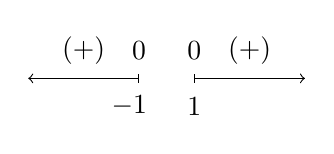
\begin{tikzpicture}[x=20pt,y=10pt]
\draw[->] (2,0) -- (0,0);
\draw[->] (3,0) -- (5,0);
\draw (2,-0.15) -- (2,0.15);
\draw (3,-0.15) -- (3,0.15);
\node at (2,-1){$-1 \hspace{7pt}$};
\node at (1,1){$(+)$};
\node at (4,1){$(+)$};
\node at (2,1){$0$};
\node at (3,1){$0$};
\node at (3,-1){$1$};
\end{tikzpicture}




Graph: \\

% \begin{mfpic}[20]{-4}{4}{-1}{4}
\axes
\tlabel[cc](4,-0.25){\scriptsize $x$}
\tlabel[cc](0.25,4){\scriptsize $y$}
\xmarks{-3,-2,-1,1,2,3}
\ymarks{1,2,3}
\tlpointsep{4pt}
\scriptsize
\axislabels {x}{{$-3 \hspace{6pt}$} -3,{$-2 \hspace{6pt}$} -2,{$-1 \hspace{6pt}$} -1, {$1$} 1, {$2$} 2, {$3$} 3}
\axislabels {y}{{$1$} 1, {$2$} 2, {$3$} 3}
\normalsize
\point[4pt]{(-1,0), (1,0)}
\dashed \polyline{(0,0), (4,4)}
\dashed \polyline{(0,0), (-4,4)}
\penwd{1.25pt}
\arrow \parafcn{0,2,0.1}{(cosh(t),sinh(t))}
\arrow \parafcn{0,2,0.1}{(-cosh(t),sinh(t))}
\end{mfpic}
\begin{tikzpicture}
\begin{axis}[
  fplot,
  xmin=-4, xmax=4, ymin=-1, ymax=4,
  width=160pt, height=100pt, scale only axis,
  xtick={-3,-2,-1,1,2,3},
  xticklabels={{$-3 \hspace{6pt}$},{$-2 \hspace{6pt}$},{$-1 \hspace{6pt}$},{ $1$},{ $2$},{ $3$}},
  ytick={1,2,3},
  yticklabels={{$1$},{$2$},{$3$}}
]
\node at (axis cs:4,-0.25){\scriptsize $x$};
\node at (axis cs:0.25,4){\scriptsize $y$};
\addplot+[only marks, mark=*, mark size=1.5pt] coordinates {(-1,0) (1,0)};
\addplot+[dashed, domain=0:4, samples=2] {x};
\addplot+[dashed, domain=-4:0, samples=2] {-x};
\addplot+[fpplot, domain=0:2, ->] ({cosh(t)},{sinh(t)});
\addplot+[fpplot, domain=0:2, ->] ({-cosh(t)},{sinh(t)});
\end{axis}
\end{tikzpicture}


Note:  $f$ is even.
\end{solution}

\end{question}

\begin{question}
$g(t) = t \sqrt{1-t^2}$
\begin{solution}
$g(t) = t\sqrt{1-t^2}$\\
Domain: $[-1,1]$\\
Intercepts: $(-1,0)$, $(0,0)$, $(1,0)$\\
Range:  $\approx [-0.5, 0.5]$\\
Local minimum $\approx (-0.707, -0.5)$ \\
Local maximum:  $\approx (0.707, 0.5)$\\
Increasing: $\approx [-0.707, 0.707]$ \\
Decreasing:  $\approx [-1, -0.707]$, $[0.707, 1]$\\
Unusual steepness at $t = -1$ and $t = 1$\\
Sign Diagram:\\

% 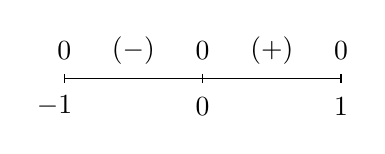
\begin{tikzpicture}[x=20pt,y=10pt]
\draw (0,0) -- (5,0);
\draw (0,-0.15) -- (0,0.15);
\draw (2.5,-0.15) -- (2.5,0.15);
\draw (5,-0.15) -- (5,0.15);
\node at (0,-1){$-1 \hspace{7pt}$};
\node at (0,1){$0$};
\node at (1.25,1){$(-)$};
\node at (2.5,-1){$0$};
\node at (3.75,1){$(+)$};
\node at (2.5,1){$0$};
\node at (5,-1){$1$};
\node at (5,1){$0$};
\end{tikzpicture}
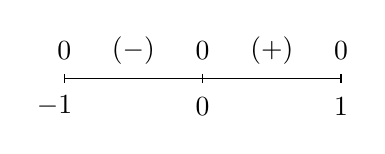
\begin{tikzpicture}[x=20pt,y=10pt]
\draw (0,0) -- (5,0);
\draw (0,-0.15) -- (0,0.15);
\draw (2.5,-0.15) -- (2.5,0.15);
\draw (5,-0.15) -- (5,0.15);
\node at (0,-1){$-1 \hspace{7pt}$};
\node at (0,1){$0$};
\node at (1.25,1){$(-)$};
\node at (2.5,-1){$0$};
\node at (3.75,1){$(+)$};
\node at (2.5,1){$0$};
\node at (5,-1){$1$};
\node at (5,1){$0$};
\end{tikzpicture}




Graph:\\

% \begin{mfpic}[50][40]{-1.5}{1.5}{-1}{1.5}
\axes
\tlabel[cc](1.5,-0.15){\scriptsize $t$}
\tlabel[cc](0.25,1.5){\scriptsize $y$}
\tlabel[cc](-1,0.15){\scriptsize $-1\hspace{7pt}$}
\tlabel[cc](0.7,0.7){\scriptsize $\approx (0.707, 0.5)$}
\tlabel[cc](-0.7,-0.7){\scriptsize $\approx (-0.707, -0.5)$}
\xmarks{-1,1}
\ymarks{-1,1}
\tlpointsep{4pt}
\scriptsize
\axislabels {x}{ {$1$} 1}
\axislabels {y}{{$1$} 1,{$-1$} -1}
\normalsize
\point[4pt]{(-1,0), (1,0),(0,0),  (-0.707, -0.5),  (0.707, 0.5)}
\penwd{1.25pt}
\parafcn{0,3.14159,0.1}{(cos(t),cos(t)*sin(t))}
\end{mfpic}
\begin{tikzpicture}
\begin{axis}[
  fplot,
  xmin=-1.5, xmax=1.5, ymin=-1, ymax=1.5,
  width=150pt, height=100pt, scale only axis,
  xtick={-1,1},
  xticklabels={,{$1$}},
  ytick={-1,1},
  yticklabels={{$-1$},{$1$}}
]
\node at (axis cs:1.5,-0.15){\scriptsize $t$};
\node at (axis cs:0.25,1.5){\scriptsize $y$};
\node at (axis cs:-1,0.15){\scriptsize $-1\hspace{7pt}$};
\node at (axis cs:0.7,0.7){\scriptsize $\approx (0.707, 0.5)$};
\node at (axis cs:-0.7,-0.7){\scriptsize $\approx (-0.707, -0.5)$};
\addplot+[only marks, mark=*, mark size=1.5pt] coordinates {(-1,0) (1,0) (0,0) (-0.707,-0.5) (0.707,0.5)};
\addplot+[fpplot, domain=0:3.14159] ({cos(t)},{cos(t)*sin(t)});
\end{axis}
\end{tikzpicture}


Note:  $g$ is odd.
\end{solution}

\end{question}

\begin{question}
$g(t) = t \sqrt{t^2-1}$

\begin{solution}
$g(t) = t\sqrt{t^2-1}$\\
Domain: $(-\infty, -1] \cup [1,\infty)$\\
Intercepts: $(-1,0)$, $(1,0)$\\
$\ds{\lim_{t \rightarrow -\infty} g(t) = -\infty}$ \\
$\ds{\lim_{t \rightarrow \infty} g(t) = \infty}$ \\
Range: $(-\infty, \infty)$\\
Increasing: $(-\infty, -1]$, $[1, \infty)$\\
Unusual steepness at $t = -1$ and $t = 1$\\
Sign Diagram:\\

\smallskip
% 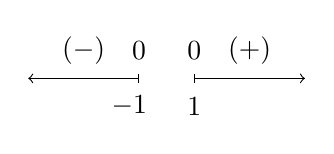
\begin{tikzpicture}[x=20pt,y=10pt]
\draw[->] (2,0) -- (0,0);
\draw[->] (3,0) -- (5,0);
\draw (2,-0.15) -- (2,0.15);
\draw (3,-0.15) -- (3,0.15);
\node at (2,-1){$-1 \hspace{7pt}$};
\node at (1,1){$(-)$};
\node at (4,1){$(+)$};
\node at (2,1){$0$};
\node at (3,1){$0$};
\node at (3,-1){$1$};
\end{tikzpicture}
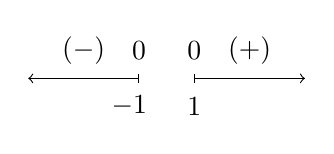
\begin{tikzpicture}[x=20pt,y=10pt]
\draw[->] (2,0) -- (0,0);
\draw[->] (3,0) -- (5,0);
\draw (2,-0.15) -- (2,0.15);
\draw (3,-0.15) -- (3,0.15);
\node at (2,-1){$-1 \hspace{7pt}$};
\node at (1,1){$(-)$};
\node at (4,1){$(+)$};
\node at (2,1){$0$};
\node at (3,1){$0$};
\node at (3,-1){$1$};
\end{tikzpicture}




Graph:\\

% \begin{tikzpicture}
\begin{axis}[
  fplot,
  xmin=-4, xmax=4, ymin=-4, ymax=4,
  width=160pt, height=120pt, scale only axis,
  xtick={-3,-2,-1,1,2,3},
  xticklabels={{$-3 \hspace{6pt}$},{$-2 \hspace{6pt}$},{$-1 \hspace{6pt}$},{ $1$},{ $2$},{ $3$}},
  ytick={-3,-2,-1,1,2,3},
  yticklabels={{$-3$},{$-2$},{$-1$},{ $1$},{ $2$},{ $3$}}
]
\node at (axis cs:4,-0.25){\scriptsize $t$};
\node at (axis cs:0.25,4){\scriptsize $y$};
\addplot+[only marks, mark=*, mark size=1.5pt] coordinates {(-1,0) (1,0)};
\addplot+[fplot, domain=-1.9:-1, <-] {x*sqrt(x^2 - 1)};
\addplot+[fplot, domain=1:1.9, ->] {x*sqrt(x^2 - 1)};
\end{axis}
\end{tikzpicture}
\begin{tikzpicture}
\begin{axis}[
  fplot,
  xmin=-4, xmax=4, ymin=-4, ymax=4,
  width=160pt, height=120pt, scale only axis,
  xtick={-3,-2,-1,1,2,3},
  xticklabels={{$-3 \hspace{6pt}$},{$-2 \hspace{6pt}$},{$-1 \hspace{6pt}$},{ $1$},{ $2$},{ $3$}},
  ytick={-3,-2,-1,1,2,3},
  yticklabels={{$-3$},{$-2$},{$-1$},{ $1$},{ $2$},{ $3$}}
]
\node at (axis cs:4,-0.25){\scriptsize $t$};
\node at (axis cs:0.25,4){\scriptsize $y$};
\addplot+[only marks, mark=*, mark size=1.5pt] coordinates {(-1,0) (1,0)};
\addplot+[fplot, domain=-1.9:-1, <-] {x*sqrt(x^2 - 1)};
\addplot+[fplot, domain=1:1.9, ->] {x*sqrt(x^2 - 1)};
\end{axis}
\end{tikzpicture}



Note:  $g$ is odd.
\end{solution}

\end{question}

\begin{question}
$f(x) = \sqrt[4]{\dfrac{16x}{x^{2} - 9}}$
\begin{solution}
$f(x) = \sqrt[4]{\dfrac{16x}{x^2 - 9}}$\\
Domain: $(-3, 0] \cup (3, \infty)$\\
Intercept: $(0,0)$\\
Range:  $[0, \infty)$\\
Decreasing: $(-3, 0]$, $(3, \infty)$\\
Unusual steepness at $x = 0$ \\
Vertical asymptotes: $x = -3$ and $x = 3$\\
Horizontal asymptote: $y = 0$\\
Sign Diagram: \\

\smallskip

% \begin{tikzpicture}[x=15pt,y=15pt]
\draw (-3,0) -- (0,0);
\draw[->] (3,0) -- (6,0);
\draw (-3,-0.1) -- (-3,0.1);
\draw (0,-0.1) -- (0,0.1);
\draw (3,-0.1) -- (3,0.1);
\node at (-1.5,0.75){$(+)$};
\node at (-3,-0.75){$-3 \hspace{7pt}$};
\node at (-3,0.75){\textinterrobang};
\node at (0,-0.75){$0$};
\node at (0,0.75){$0$};
\node at (3,0.75){\textinterrobang};
\node at (3,-0.75){$3$};
\node at (4.5,0.75){$(+)$};
\end{tikzpicture}
\begin{tikzpicture}[x=15pt,y=15pt]
\draw (-3,0) -- (0,0);
\draw[->] (3,0) -- (6,0);
\draw (-3,-0.1) -- (-3,0.1);
\draw (0,-0.1) -- (0,0.1);
\draw (3,-0.1) -- (3,0.1);
\node at (-1.5,0.75){$(+)$};
\node at (-3,-0.75){$-3 \hspace{7pt}$};
\node at (-3,0.75){\textinterrobang};
\node at (0,-0.75){$0$};
\node at (0,0.75){$0$};
\node at (3,0.75){\textinterrobang};
\node at (3,-0.75){$3$};
\node at (4.5,0.75){$(+)$};
\end{tikzpicture}





Graph:\\
% \begin{mfpic}[15]{-3.5}{9}{-1}{6}
\axes
\tlabel[cc](9,-0.5){\scriptsize $x$}
\tlabel[cc](0.5,6){\scriptsize $y$}
\xmarks{-3 step 1 until 8}
\ymarks{1,2,3,4,5}
\tlpointsep{4pt}
\scriptsize
\axislabels {x}{{$-3 \hspace{6pt}$} -3, {$-2 \hspace{6pt}$} -2, {$-1 \hspace{6pt}$} -1, {$1$} 1, {$2$} 2, {$3$} 3, {$4$} 4, {$5$} 5, {$6$} 6, {$7$} 7, {$8$} 8}
\axislabels {y}{{$1$} 1, {$2$} 2, {$3$} 3, {$4$} 4, {$5$} 5}
\normalsize
\point[4pt]{(0,0)}
\dashed \polyline{(-3,-1), (-3,6)}
\dashed \polyline{(3,-1), (3,6)}
\penwd{1.25pt}
\arrow \reverse \function{-2.93,0,0.1}{((16*x)/((x**2) - 9))**(0.25)}
\arrow \reverse \arrow \function{3.05,9,0.1}{((16*x)/((x**2) - 9))**(0.25)}
\end{mfpic}
\begin{tikzpicture}
\begin{axis}[
  fplot,
  xmin=-3.5, xmax=9, ymin=-1, ymax=6,
  width=187.5pt, height=105pt, scale only axis,
  xtick={-3,-2,-1,0,1,2,3,4,5,6,7,8},
  xticklabels={{$-3 \hspace{6pt}$},{$-2 \hspace{6pt}$},{$-1 \hspace{6pt}$},,{$1$},{$2$},{$3$},{$4$},{$5$},{$6$},{$7$},{$8$}},
  ytick={1,2,3,4,5},
  yticklabels={{$1$},{$2$},{$3$},{$4$},{$5$}}
]
\node at (axis cs:9,-0.5){\scriptsize $x$};
\node at (axis cs:0.5,6){\scriptsize $y$};
\addplot+[only marks, mark=*, mark size=1.5pt] coordinates {(0,0)};
\addplot+[dashed] coordinates {(-3,-1) (-3,6)};
\addplot+[dashed] coordinates {(3,-1) (3,6)};
\addplot+[fplot, domain=-2.93:0, <-] {( (16*x)/((x^2) - 9) )^(0.25)};
\addplot+[fplot, domain=3.05:9, <->] {( (16*x)/((x^2) - 9) )^(0.25)};
\end{axis}
\end{tikzpicture}
\end{solution}

\end{question}

\begin{question}
$f(x) = \dfrac{5x}{\sqrt[3]{x^{3} + 8}}$
\begin{solution}
$f(x) = \dfrac{5x}{\sqrt[3]{x^{3} + 8}}$\\
Domain: $(-\infty, -2) \cup (-2, \infty)$\\
Intercept:  $(0,0)$\\
Range:  $(-\infty, 5) \cup (5, \infty)$\\
Increasing: $(-\infty, -2)$, $(-2, \infty)$\\
Vertical asymptote $x = -2$\\
Horizontal asymptote $y = 5$\\
Sign Diagram:\\ 

\smallskip

% \begin{mfpic}[20]{-4}{2}{-1}{1}
\arrow \reverse \arrow \polyline{(-4,0),(2,0)}
\xmarks{-2,0}
\tlabel[cc](-3, 0.5){$(+)$}
\tlabel[cc](-2,-0.5){$-2 \hspace{7pt}$}
\tlabel[cc](-2,0.5){\textinterrobang}
\tlabel[cc](-1,0.5){$(-)$}
\tlabel[cc](0,-0.5){$0$}
\tlabel[cc](0,0.5){$0$}
\tlabel[cc](1,0.5){$(+)$}
\end{mfpic}
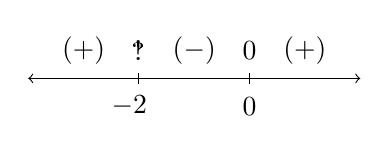
\begin{tikzpicture}[x=20pt,y=20pt]
\draw[<->] (-4,0) -- (2,0);
\draw (-2,-0.1) -- (-2,0.1);
\draw (0,-0.1) -- (0,0.1);
\node at (-3, 0.5){$(+)$};
\node at (-2,-0.5){$-2 \hspace{7pt}$};
\node at (-2,0.5){\textinterrobang};
\node at (-1,0.5){$(-)$};
\node at (0,-0.5){$0$};
\node at (0,0.5){$0$};
\node at (1,0.5){$(+)$};
\end{tikzpicture}




Graph: \\

% \begin{mfpic}[10][8]{-5}{5}{-7}{9}
\axes
\tlabel[cc](5,-0.5){\scriptsize $x$}
\tlabel[cc](0.5,9){\scriptsize $y$}
\xmarks{-4 step 1 until 4}
\ymarks{-6 step 1 until 8}
\tlpointsep{4pt}
\tiny
\axislabels {x}{{$-4 \hspace{6pt}$} -4, {$-3 \hspace{6pt}$} -3, {$-2 \hspace{6pt}$} -2, {$-1 \hspace{6pt}$} -1, {$1$} 1, {$2$} 2, {$3$} 3, {$4$} 4}
\axislabels {y}{{$-6$} -6, {$-5$} -5, {$-4$} -4, {$-3$} -3,{$1$} 1, {$2$} 2, {$3$} 3, {$4$} 4, {$5$} 5, {$6$} 6, {$7$} 7, {$8$} 8}
\normalsize
\dashed \polyline{(-5,5), (5,5)}
\dashed \polyline{(-2,-7), (-2,9)}
\point[4pt]{(0,0)}
\penwd{1.25pt}
\arrow \reverse \arrow \function{-5,-2.2,0.1}{(-5*x)/((-(x**3) - 8)**(1/3))}
\arrow \reverse \arrow \function{-1.8,5,0.1}{(5*x)/(((x**3) + 8)**(1/3))}
\end{mfpic}
\begin{tikzpicture}
\begin{axis}[
  fplot,
  xmin=-5, xmax=5, ymin=-7, ymax=9,
  width=100pt, height=128pt, scale only axis,
  xtick={-4,-3,-2,-1,1,2,3,4},
  xticklabels={{$-4 \hspace{6pt}$},{$-3 \hspace{6pt}$},{$-2 \hspace{6pt}$},{$-1 \hspace{6pt}$},{ $1$},{ $2$},{ $3$},{ $4$}},
  ytick={-6,-5,-4,-3,-2,-1,0,1,2,3,4,5,6,7,8},
  yticklabels={{$-6$},{$-5$},{$-4$},{$-3$},,,,{ $1$},{ $2$},{ $3$},{ $4$},{ $5$},{ $6$},{ $7$},{ $8$}}
]
\node at (axis cs:5,-0.5){\scriptsize $x$};
\node at (axis cs:0.5,9){\scriptsize $y$};
\addplot+[dashed, domain=-5:5, samples=2] {5};
\addplot+[dashed] coordinates {(-2,-7) (-2,9)};
\addplot+[only marks, mark=*, mark size=1.5pt] coordinates {(0,0)};
\addplot+[fplot, domain=-5:-2.2, <->] {(-5*x)/( (abs(-(x^3) - 8))^(1/3) * sign(-(x^3) - 8) )};
\addplot+[fplot, domain=-1.8:5, <->] {(5*x)/( (abs((x^3) + 8))^(1/3) * sign((x^3) + 8) )};
\end{axis}
\end{tikzpicture}
\end{solution}

\end{question}

\begin{question}
$g(t) = \sqrt{t(t + 5)(t - 4)}$
\begin{solution}
$g(t) = \sqrt{t(t + 5)(t - 4)}$\\
Domain: $[-5, 0] \cup [4, \infty)$\\
Intercepts  $(-5,0)$, $(0,0)$, $(4,0)$\\
$\ds{\lim_{t \rightarrow \infty} g(t) = \infty}$\\
Range:  $[0, \infty)$\\
Local maximum $\approx (-2.937, 6.483)$\\
Increasing: $\approx [-5, -2.937]$, $[4, \infty)$\\
Decreasing: $\approx [-2.937,0]$\\
Unusual steepness at $t = -5, t = 0$ and $t = 4$\\
Sign Diagram:\\

\smallskip

% \begin{mfpic}[10]{-5}{8}{-1}{1}
\polyline{(-5,0),(0,0)}
\arrow  \polyline{(4,0),(8,0)}
\xmarks{-5,0,4}
\tlabel[cc](-5,-1){$-5 \hspace{7pt}$}
\tlabel[cc](-5,1){$0$}
\tlabel[cc](-2.5,1){$(+)$}
\tlabel[cc](0,-1){$0$}
\tlabel[cc](0,1){$0$}
\tlabel[cc](4,-1){$4$}
\tlabel[cc](4,1){$0$}
\tlabel[cc](6,1){$(+)$}
\end{mfpic}
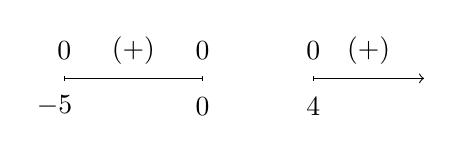
\begin{tikzpicture}[x=10pt,y=10pt]
\draw (-5,0) -- (0,0);
\draw[->] (4,0) -- (8,0);
\draw (-5,-0.1) -- (-5,0.1);
\draw (0,-0.1) -- (0,0.1);
\draw (4,-0.1) -- (4,0.1);
\node at (-5,-1){$-5 \hspace{7pt}$};
\node at (-5,1){$0$};
\node at (-2.5,1){$(+)$};
\node at (0,-1){$0$};
\node at (0,1){$0$};
\node at (4,-1){$4$};
\node at (4,1){$0$};
\node at (6,1){$(+)$};
\end{tikzpicture}




Graph:\\
% \begin{tikzpicture}
\begin{axis}[
  fplot,
  xmin=-6, xmax=6, ymin=-1, ymax=10,
  width=120pt, height=110pt, scale only axis,
  xtick={-5,-4,-3,-2,-1,1,2,3,4,5},
  xticklabels={{$-5 \hspace{6pt}$},{$-4 \hspace{6pt}$},{$-3 \hspace{6pt}$},{$-2 \hspace{6pt}$},{$-1 \hspace{6pt}$},{ $1$},{ $2$},{ $3$},{ $4$},{ $5$}},
  ytick={1,2,3,4,5,6,7,8,9},
  yticklabels={{$1$},{$2$},{$3$},{$4$},{$5$},{$6$},,{$8$},{$9$}}
]
\node at (axis cs:6,-0.5){\scriptsize $t$};
\node at (axis cs:0.5,10){\scriptsize $y$};
\node at (axis cs:-3.5,7){\scriptsize $\approx (-2.937, 6.483)$};
\addplot+[only marks, mark=*, mark size=1.5pt] coordinates {(-5,0) (0,0) (4,0) (-2.937,6.483)};
\addplot+[fplot, domain=-5:0] {sqrt(x^3 + x^2 - 20*x)};
\addplot+[fplot, domain=4:5.5, ->] {sqrt(x^3 + x^2 - 20*x)};
\end{axis}
\end{tikzpicture}
\begin{tikzpicture}
\begin{axis}[
  fplot,
  xmin=-6, xmax=6, ymin=-1, ymax=10,
  width=120pt, height=110pt, scale only axis,
  xtick={-5,-4,-3,-2,-1,1,2,3,4,5},
  xticklabels={{$-5 \hspace{6pt}$},{$-4 \hspace{6pt}$},{$-3 \hspace{6pt}$},{$-2 \hspace{6pt}$},{$-1 \hspace{6pt}$},{ $1$},{ $2$},{ $3$},{ $4$},{ $5$}},
  ytick={1,2,3,4,5,6,7,8,9},
  yticklabels={{$1$},{$2$},{$3$},{$4$},{$5$},{$6$},,{$8$},{$9$}}
]
\node at (axis cs:6,-0.5){\scriptsize $t$};
\node at (axis cs:0.5,10){\scriptsize $y$};
\node at (axis cs:-3.5,7){\scriptsize $\approx (-2.937, 6.483)$};
\addplot+[only marks, mark=*, mark size=1.5pt] coordinates {(-5,0) (0,0) (4,0) (-2.937,6.483)};
\addplot+[fplot, domain=-5:0] {sqrt(x^3 + x^2 - 20*x)};
\addplot+[fplot, domain=4:5.5, ->] {sqrt(x^3 + x^2 - 20*x)};
\end{axis}
\end{tikzpicture}
\end{solution}

\end{question}

\begin{question}
$g(t) = \sqrt[3]{t^{3} + 3t^{2} - 6t - 8}$ 

\begin{solution}
$g(t) = \sqrt[3]{t^{3} + 3t^{2} - 6t - 8}$\\
Domain: $(-\infty, \infty)$\\
Intercepts:  $(-4,0)$, $(-1,0)$, $(0,-2)$, $(2,0)$\\
\footnote{Using Calculus it can be shown that $y = t + 1$ is a slant asymptote of this graph.}$\ds{\lim_{t \rightarrow -\infty} g(t) = -\infty}$\\
$\ds{\lim_{t \rightarrow \infty} g(t) = \infty}$\\
Range:  $(-\infty, \infty)$\\
Local maximum:  $\approx (-2.732, 2.182)$\\
Local minimum:  $\approx (0.732, -2.182)$\\
Increasing:  $\approx (-\infty, -2.732]$, $[0.732, \infty)$\\
Decreasing: $\approx [-2.732, 0.732]$\\
Unusual steepness at $t = -4, t = -1$ and $t = 2$\\




Sign Diagram:\\

% \begin{mfpic}[10]{-8}{6}{-1}{1}
\arrow \reverse \arrow \polyline{(-8,0),(6,0)}
\xmarks{-4,-1,2}
\tlabel[cc](-6,1){$(-)$}
\tlabel[cc](-4,-1){$-4 \hspace{7pt}$}
\tlabel[cc](-4,1){$0$}
\tlabel[cc](-2.5,1){$(+)$}
\tlabel[cc](-1,-1){$-1 \hspace{7pt}$}
\tlabel[cc](-1,1){$0$}
\tlabel[cc](0.5,1){$(-)$}
\tlabel[cc](2,-1){$2$}
\tlabel[cc](2,1){$0$}
\tlabel[cc](4,1){$(+)$}
\end{mfpic}
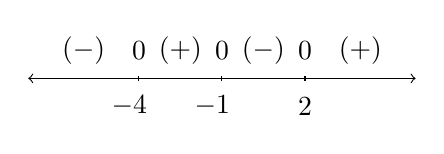
\begin{tikzpicture}[x=10pt,y=10pt]
\draw[<->] (-8,0) -- (6,0);
\draw (-4,-0.1) -- (-4,0.1);
\draw (-1,-0.1) -- (-1,0.1);
\draw (2,-0.1) -- (2,0.1);
\node at (-6,1){$(-)$};
\node at (-4,-1){$-4 \hspace{7pt}$};
\node at (-4,1){$0$};
\node at (-2.5,1){$(+)$};
\node at (-1,-1){$-1 \hspace{7pt}$};
\node at (-1,1){$0$};
\node at (0.5,1){$(-)$};
\node at (2,-1){$2$};
\node at (2,1){$0$};
\node at (4,1){$(+)$};
\end{tikzpicture}




Graph:\\
% \begin{tikzpicture}
\begin{axis}[
  fplot,
  xmin=-6, xmax=6, ymin=-5, ymax=7,
  width=120pt, height=120pt, scale only axis,
  xtick={-5,-4,-3,-2,-1,0,1,2,3,4,5},
  xticklabels={{$-5 \hspace{6pt}$},,{$-3 \hspace{6pt}$},{$-2 \hspace{6pt}$},,,{ $1$},,{$3$},{ $4$},{ $5$}},
  ytick={-4,-3,-2,-1,0,1,2,3,4,5,6},
  yticklabels={{$-4$},{$-3$},{$-2$},{$-1$},,{$1$},{$2$},{$3$},{$4$},{$5$},{$6$}}
]
\node at (axis cs:6,-0.5){\scriptsize $t$};
\node at (axis cs:0.5,7){\scriptsize $y$};
\node at (axis cs:-4,3){\scriptsize $\approx (-2.732, 2.182)$};
\node at (axis cs:3.25,-2.75){\scriptsize $\approx (0.732, -2.182)$};
\addplot+[only marks, mark=*, mark size=1.5pt] coordinates {(-4,0) (-1,0) (2,0) (-2.732,2.182) (0.732,-2.182)};
\addplot+[dashed, domain=-6:6, samples=2] {x};
\addplot+[fplot, domain=-6:-4, <-] { - ( - ( (x^3) + 3*(x^2) - 6*x - 8 ) )^(1/3) };
\addplot+[fplot, domain=-4:-1] { (abs((x^3) + 3*(x^2) - 6*x - 8))^(1/3) * sign((x^3) + 3*(x^2) - 6*x - 8) };
\addplot+[fplot, domain=-1:2] { - (abs((x^3) + 3*(x^2) - 6*x - 8))^(1/3) * sign((x^3) + 3*(x^2) - 6*x - 8) };
\addplot+[fplot, domain=2:6, ->] { (abs((x^3) + 3*(x^2) - 6*x - 8))^(1/3) * sign((x^3) + 3*(x^2) - 6*x - 8) };
\end{axis}
\end{tikzpicture}
\begin{tikzpicture}
\begin{axis}[
  fplot,
  xmin=-6, xmax=6, ymin=-5, ymax=7,
  width=120pt, height=120pt, scale only axis,
  xtick={-5,-4,-3,-2,-1,0,1,2,3,4,5},
  xticklabels={{$-5 \hspace{6pt}$},,{$-3 \hspace{6pt}$},{$-2 \hspace{6pt}$},,,{ $1$},,{$3$},{ $4$},{ $5$}},
  ytick={-4,-3,-2,-1,0,1,2,3,4,5,6},
  yticklabels={{$-4$},{$-3$},{$-2$},{$-1$},,{$1$},{$2$},{$3$},{$4$},{$5$},{$6$}}
]
\node at (axis cs:6,-0.5){\scriptsize $t$};
\node at (axis cs:0.5,7){\scriptsize $y$};
\node at (axis cs:-4,3){\scriptsize $\approx (-2.732, 2.182)$};
\node at (axis cs:3.25,-2.75){\scriptsize $\approx (0.732, -2.182)$};
\addplot+[only marks, mark=*, mark size=1.5pt] coordinates {(-4,0) (-1,0) (2,0) (-2.732,2.182) (0.732,-2.182)};
\addplot+[dashed, domain=-6:6, samples=2] {x};
\addplot+[fplot, domain=-6:-4, <-] { - ( - ( (x^3) + 3*(x^2) - 6*x - 8 ) )^(1/3) };
\addplot+[fplot, domain=-4:-1] { (abs((x^3) + 3*(x^2) - 6*x - 8))^(1/3) * sign((x^3) + 3*(x^2) - 6*x - 8) };
\addplot+[fplot, domain=-1:2] { - (abs((x^3) + 3*(x^2) - 6*x - 8))^(1/3) * sign((x^3) + 3*(x^2) - 6*x - 8) };
\addplot+[fplot, domain=2:6, ->] { (abs((x^3) + 3*(x^2) - 6*x - 8))^(1/3) * sign((x^3) + 3*(x^2) - 6*x - 8) };
\end{axis}
\end{tikzpicture}






\end{solution}

\end{question}

\begin{question}
Rework Example \ref{SasquatchCable} so that the outpost is 10 miles from Route 117 and the nearest junction box is 30 miles down the road for the post.
\begin{solution}
$C(x) = 15x+20\sqrt{100+(30-x)^2}$, $0 \leq x \leq 30$.  The calculator gives the absolute minimum at approximately $(18.66, 582.29)$.  This means to minimize the cost, approximately 18.66 miles of cable should be run along Route 117 before turning off the road and heading towards the outpost.  The minimum cost to run the cable is approximately $\$582.29$.
\end{solution}

\end{question}

\begin{question}
The volume $V$ of a right cylindrical cone depends on the radius of its base $r$ and its height $h$ and is given by the formula $V = \frac{1}{3} \pi r^2 h$.  The surface area $S$ of a right cylindrical cone also depends on $r$ and $h$ according to the formula $S = \pi r \sqrt{r^2+h^2}$.  In the following problems, suppose a cone is to have a volume of 100 cubic centimeters. 

\begin{solution}
\end{solution}

\end{question}

\begin{question}
Use the formula for volume to find the height as a function of $r$, $h(r)$.
\begin{solution}
$h(r) = \frac{300}{\pi r^2}$, $r > 0$.
\end{solution}

\end{question}

\begin{question}
Use the formula for surface area along with  your answer to \ref{heightintermsofr} to find the surface area as a function of $r$, $S(r)$.
\begin{solution}
$S(r) = \pi r \sqrt{r^2+\left(\frac{300}{\pi r^2}\right)^2} = \frac{\sqrt{\pi^2 r^6+90000}}{r}$, $r>0$
\end{solution}

\end{question}

\begin{question}
Use your calculator to find the values of $r$ and $h$ which minimize the surface area.  What is the minimum surface area?  Round your answers to two decimal places.
\begin{solution}
The calculator gives the absolute minimum at the point $\approx (4.07, 90.23)$.  This means the radius should be (approximately) 4.07 centimeters and the height should be 5.76 centimeters to give a minimum surface area of 90.23 square centimeters.
\end{solution}

\end{question}

\begin{question}
Find the applied domain of the function.
\begin{solution}
$[0, c)$
\end{solution}

\end{question}

\begin{question}
Compute $m(.1c), \, m(.5c), \, m(.9c)$ and $m(.999c)$.
\begin{solution}
$m(.1c) = \dfrac{m_{r}}{\sqrt{.99}} \approx 1.005m_{r}$,  $m(.5c) = \dfrac{m_{r}}{\sqrt{.75}} \approx 1.155m_{r}$,  $m(.9c) = \dfrac{m_{r}}{\sqrt{.19}} \approx 2.294m_{r}$, $m(.999c) = \dfrac{m_{r}}{\sqrt{.0.001999}} \approx 22.366m_{r}$.
\end{solution}

\end{question}

\begin{question}
Find $\ds{\lim_{v \rightarrow c^{-}} m(v)}$.
\begin{solution}
$\ds{\lim_{v \rightarrow c^{-}} m(x) \rightarrow \infty}$;   as the object's velocity approaches the speed of light, mass becomes infinite.
\end{solution}

\end{question}

\begin{question}
How slowly must the object be traveling so that the observed mass is no greater than 100 times its mass at rest?
\begin{solution}
If the object is traveling no faster than approximately $0.99995$ times the speed of light, then its observed mass will be no greater than $100m_{r}$.
\end{solution}

\end{question}

\end{document}